\subsection{第 10 课 | 贪心算法}

贪心算法是一种在每一步选择中都采取在当前状态下最好或最优(即最有
利)的选择,从而希望导致结果是全局最好或最优的算法。

贪心算法与动态规划的不同在于它对每个子问题的解决方案都做出选择,不
能回退。动态规划则会保存以前的运算结果,并根据以前的结果对当前进行
选择,有回退功能。

贪心法可以解决一些最优化问题,如:求图中的最小生成树、求哈夫曼编码
等。然而对于工程和生活中的问题,贪心法一般不能得到我们所要求的答
案。

一旦一个问题可以通过贪心法来解决,那么贪心法一般是解决这个问题的最
好办法。由于贪心法的高效性以及其所求得的答案比较接近最优结果,贪心
法也可以用作辅助算法或者直接解决一些要求结果不特别精确的问题。

\subsubsection{脑图}

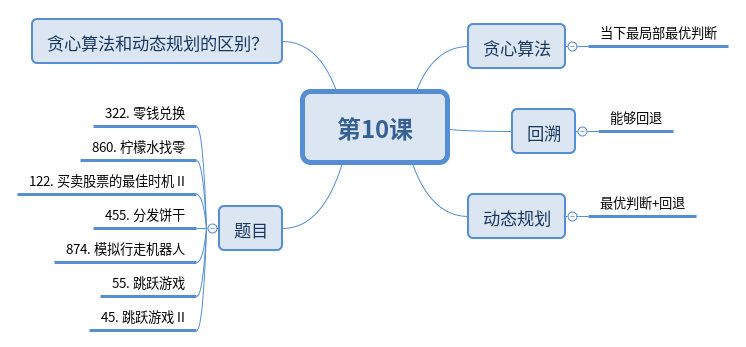
\includegraphics[width=170mm,height=80mm]{images/camp/第10课.png}

\subsubsection{题目}

\begin{itemize}
  \item \hyperref[leetcode:322]{322. 零钱兑换}
  \item \hyperref[leetcode:860]{860. 柠檬水找零}
  \item \hyperref[leetcode:122]{122. 买卖股票的最佳时机 II}
  \item \hyperref[leetcode:455]{455. 分发饼干}
  \item \hyperref[leetcode:874]{874. 模拟行走机器人}
  \item \hyperref[leetcode:55]{55. 跳跃游戏}
  \item \hyperref[leetcode:45]{45. 跳跃游戏 II}
\end{itemize}
